\documentclass[twocolumn, aps, apl]{revtex4-1}

\usepackage{graphicx}
\usepackage{fancyhdr}
\usepackage{amsmath}
\usepackage{caption}
\usepackage{enumerate}
\usepackage{subcaption}
\usepackage{textcomp}
\usepackage{placeins}

\begin{document}
\title{Lab 2. Passive Elements: Power Dividers and Impedance Matching }
\author{Albert Wandui}
\affiliation{EE 152: High Frequency Systems Lab.}
\maketitle

\section*{Introduction}
The goal of this lab was to design, provide fabrication outputs and characterize passive microwave circuits. We designed a Branch Line Coupler and a Wilkinson Power Divider using Microwave Office (MWO). In addition, we matched an RC load to a 50 $\Omega$ line at 4GHz. Power couplers and dividers have numerous applications in the microwave and RF regimes. Branch Line couplers.


\section*{Branch Line Coupler}

\subsection{Design}
The Branch Line Coupler is a 4 port circuit that divides power equally between 2 output ports with phase offsets between the input and outputs ports. The final port (4) is the isolation port and receives no power from the input. The phase at port 2 (output 1) is 90\textdegree offset from the input and that of port 3 (output 2) is 180 \textdegree offset from the input. A schematic of a branch line coupler is shown below ADDFIGURE. The branch lines are spaced at a distance of $\lambda/2$ from the two main transmission line trunks. 

The branch line coupler can be analyzed using Even and Odd Mode Analysis. The impedance of the branch is $Z_0$ while that of the main line is $Z_1$. For the even mode, we assume that +V volts are applied at both port 1 and port 4. In this case, there is no potential difference across the branches and therefore no current. We can thus split the circuit into 2 across the middle symmetry line by placing open circuit terminations at the ends of the half branches. In addition, we terminate the output ports by resistors equal to the characteristic impedance $Z_0$. In the resulting half circuit, there are reflections at the 2 contacts between the $Z_0$ and $Z_1$ transmission lines. 


For impedance of the branch lines equal to 50 $\Omega$ that of the main transmission line will be $\sqrt{50 \times 100}$ = 35.56 $\Omega$. 

For this lab, all the transmission lines were microstrip made out of 35 $\mu$m thick copper deposited on 50 mils of Rodgers RO3210 which has a dielectric constant of 10.2 and loss tangent 0.0027. The widths of the microstrip lines for the desired characteristic impedances were calculated using the TXLine program in Microwave Office. The lengths of the quarter wavelength sections were also computed in the same way. The table \ref{tab:branch} summarizes the dimensions of the Branch Line Coupler after the circuit was optimized for power transmission at 5.9 GHz. After tuning, the designed circuit coupled -3.145 dB of power to port 2 and -3.137 dB to port 3 with -20 dB isolation on port 4 as shown in figure \ref{fig:branchmag}.

\begin{tabular}{l | c | c}
    \hline
    Z [$\Omega$] & W [mils] & $\lambda/4$ [mils] \\
    \hline
    50  & 44.5 & 175.0 \\
    35.36 & 73.5 & 167.5 \\
    \hline
% \caption{Parameters of the transmission lines used in the branch line coupler. All dimensions have been rounded to the nearest half mil and the values reported are the optimized values to center the circuit response at 5.9 GHz. }
% \label{tab:branch}
\end{tabular}

Using the circuit design, we made a layout and routed the input and output lines to fit the 1x1 inch circuit size. The spacing between the input and output traces was set to about 500 mils for ease of mounting the SMA connectors. 

\subsection{Lab Testing and Analysis}
In lab, we soldered the SMA connectors to the input and output traces of the circuit after deburring the edges of the fabricated circuit for a snug fit. We then calibrated the FieldFox Network Analyzer with the input power set to -10.0 dBm. Once calibration was done, we measured 3 2-port responses of the branch line coupler; $S_{21}, S_{31}$ and $S_{41}$. The results in comparison to the simulated circuit response are shown in figure \ref{fig:branchmag} and \ref{fig:branchphase}. 

From the figure, we can see clear deviations in the measured vs. simulated response of the circuit. There are a number of possible explanations for these effects. For starters, the solder joints between the SMA launches and the circuit could introduce unwanted impedances into the circuit. Capacitive and Inductive connections would modify the circuit response. ADDSECTION.

Some of the deviations could also be explained by the tolerances in the fabrication of the circuit. The substrate material datasheet lists 2 different values for the dielectric constant as measured by different techniques. Setting the dielectric constant in the range 10.2 - 10.8 gives trace widths in the range ADDVALUE and quarter wavelength ranges ADDVALUE for the 50 $\Omega$ sections. This could change the response of the circuit as shown below. 

We tested these hypotheses by varying the coupler line widths to make simulations that matched the measured results. The results are shown in figure ADDFIGURE. 


% \begin{figure}[!htbp]
%     \centering
%     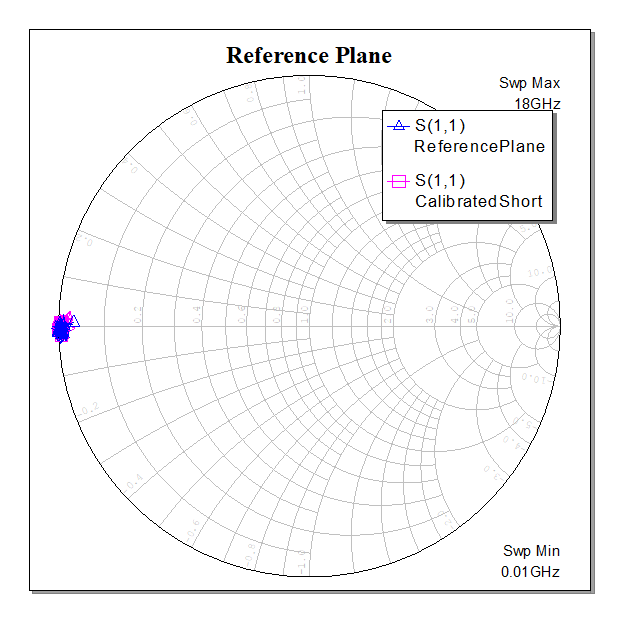
\includegraphics[scale=0.5]{CalibratedShort.png}
%     \caption{Smith Chart showing the Short Calibration Standard with Reference Plane Extensions done on the NA (purple) and emulated on Microwave Office (blue).}
%     \label{fig:calib}
% \end{figure}

\FloatBarrier

\section*{Wilkinson Power Divider}

\subsection{Design}

\subsection{Lab Testing and Analysis}


% \begin{figure}[!htbp]
%     \centering
%     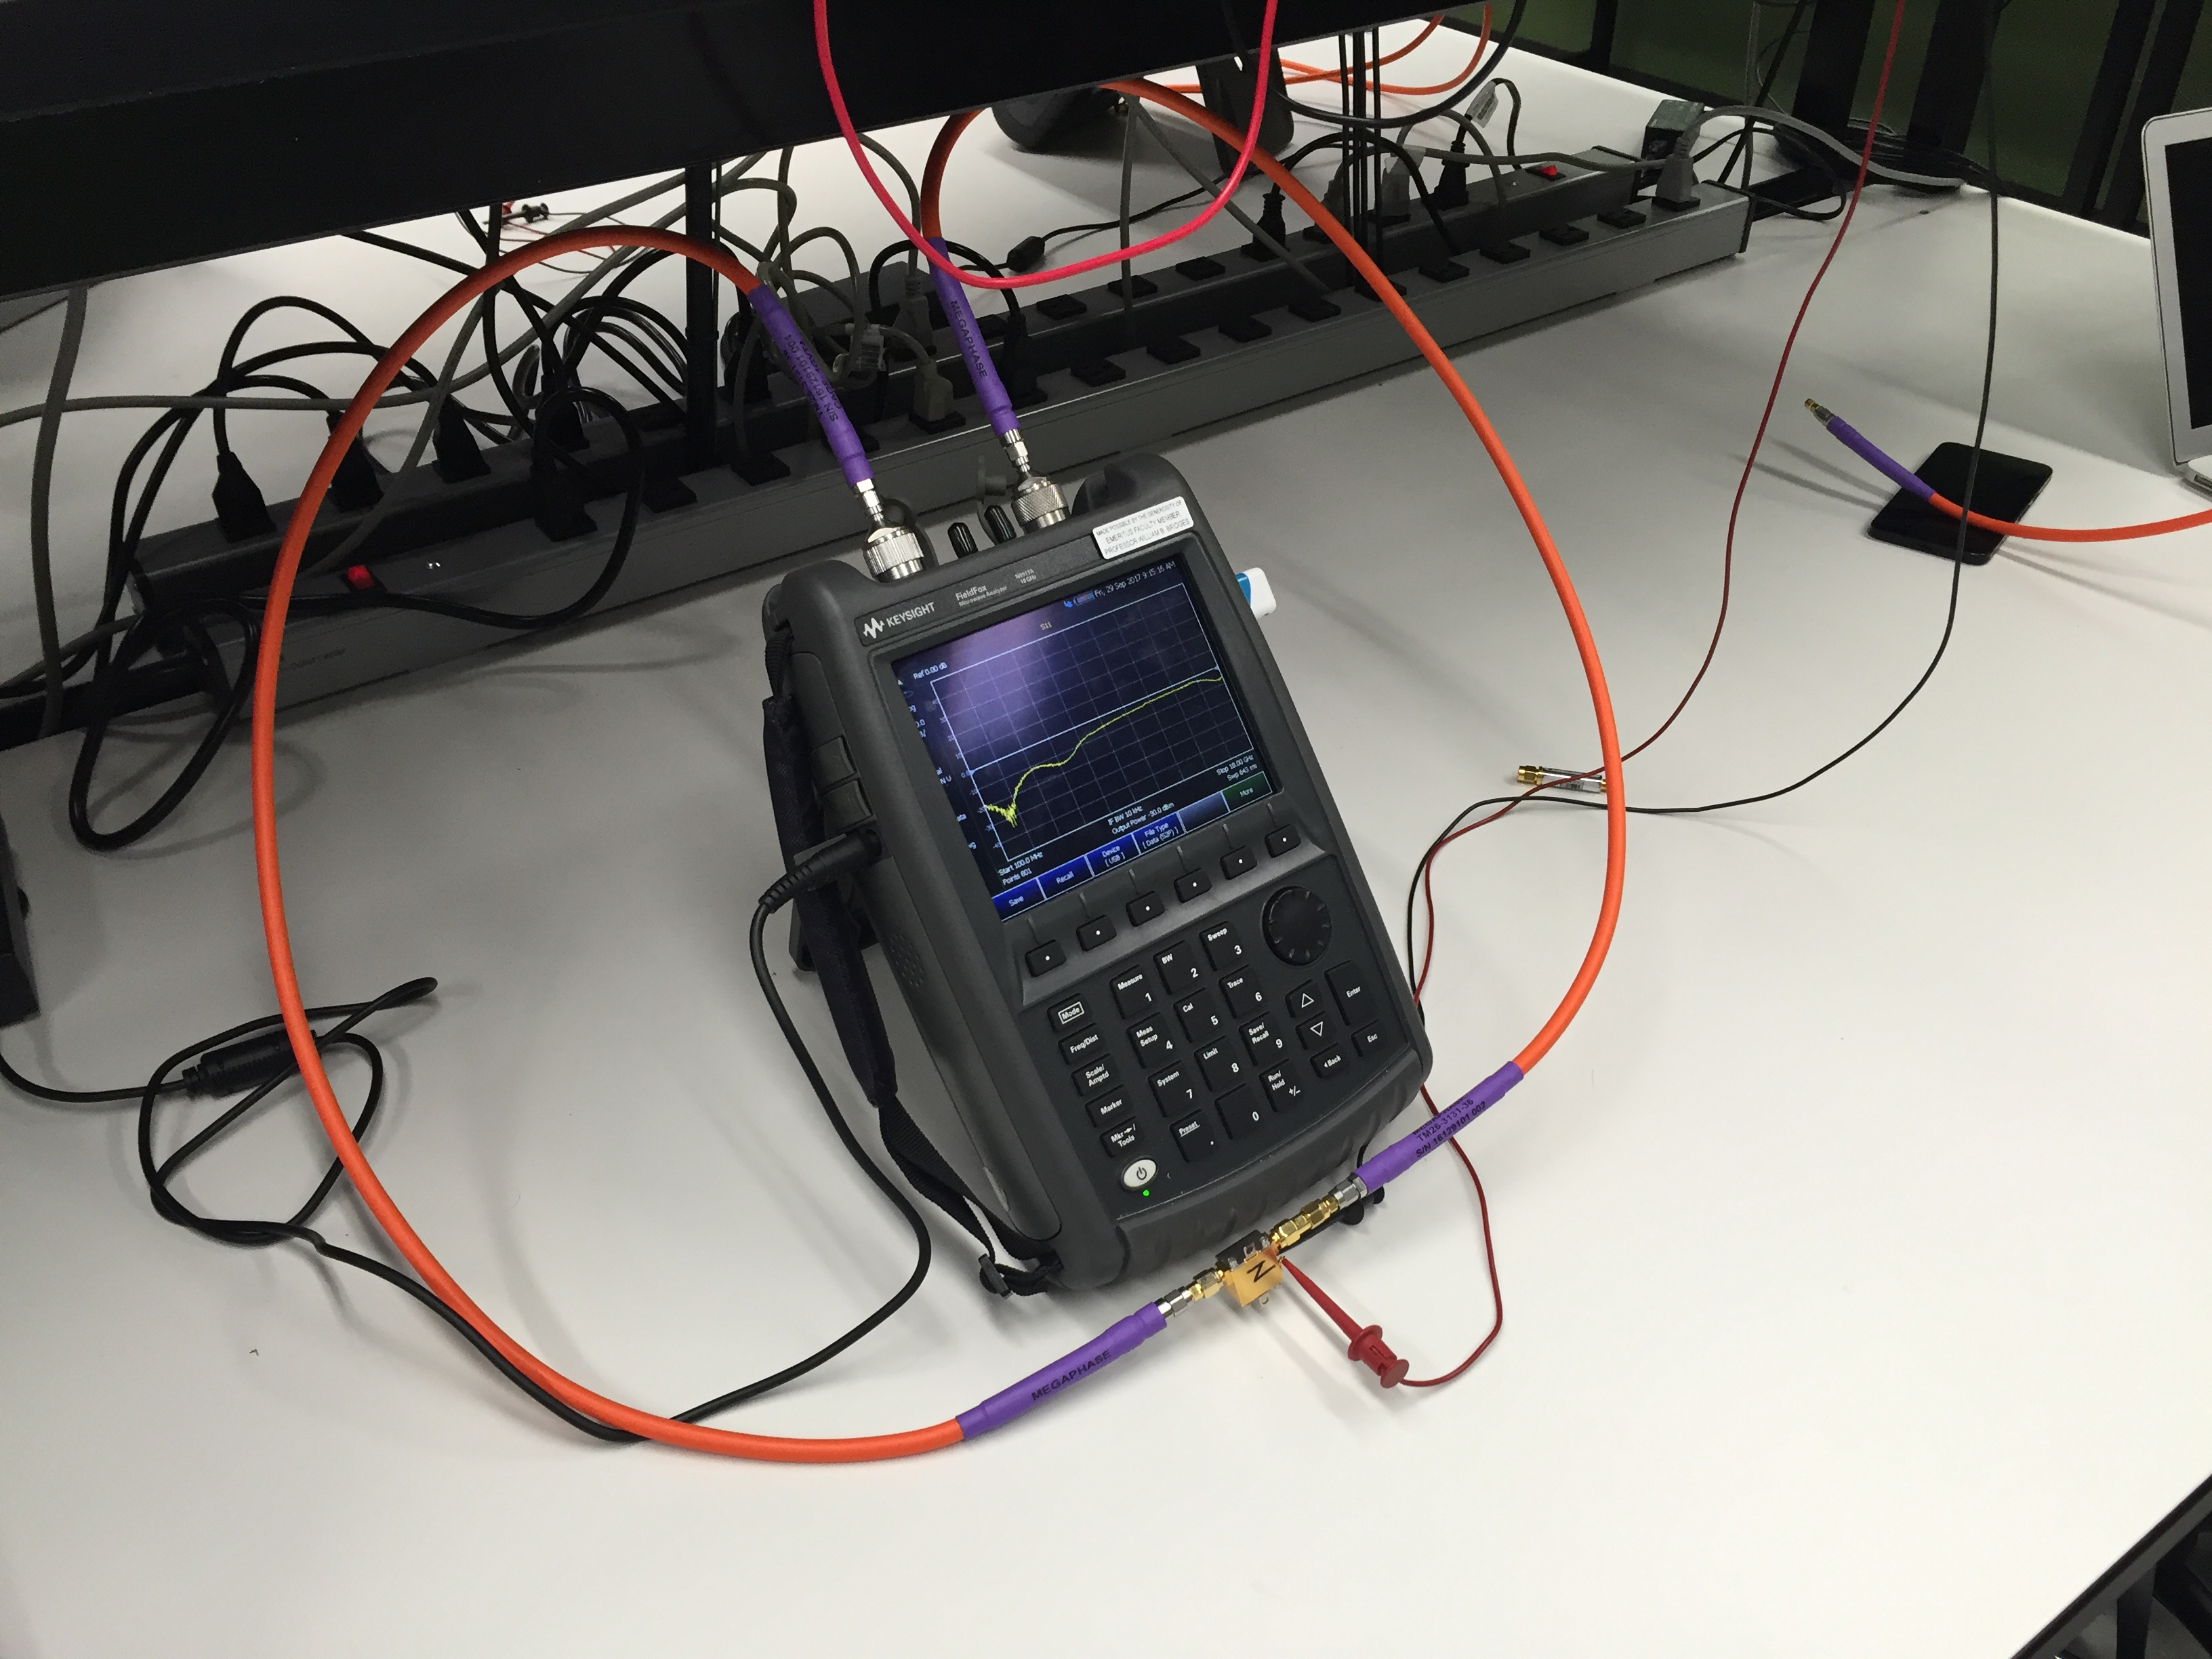
\includegraphics[width=0.35\textwidth]{amp_measurement.jpeg}
%     \caption{Measurement Setup for amplifier on the NA.}
%     \label{fig:ampimg}
% \end{figure}


% \begin{figure}[!htbp]
%     \centering
%     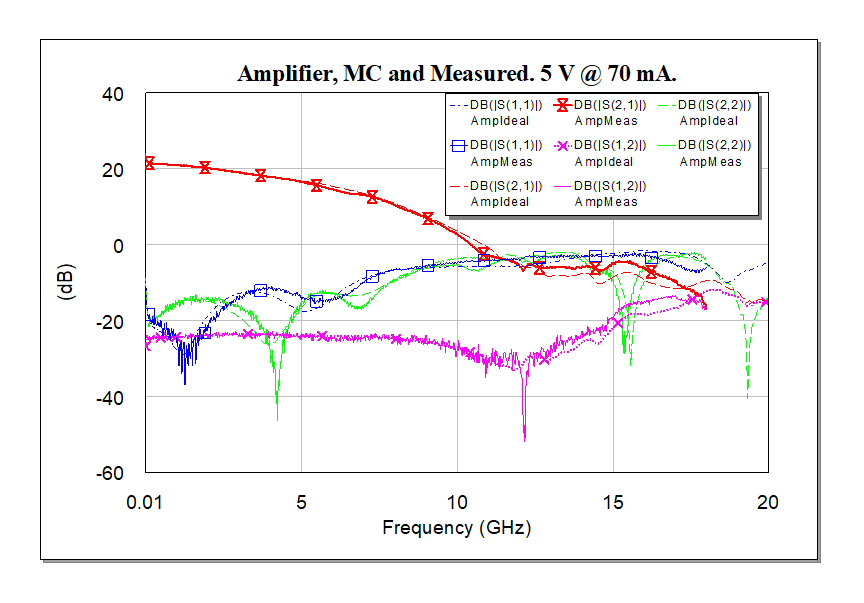
\includegraphics[scale=0.45]{AmplifierMCandMeasured.png}
%     \caption{Comparison of the Amplifier S parameters from the NA measurements to the sourced values from the data sheet.}
%     \label{fig:amp}
% \end{figure}


% \begin{figure}[!htbp]
%     \centering
%     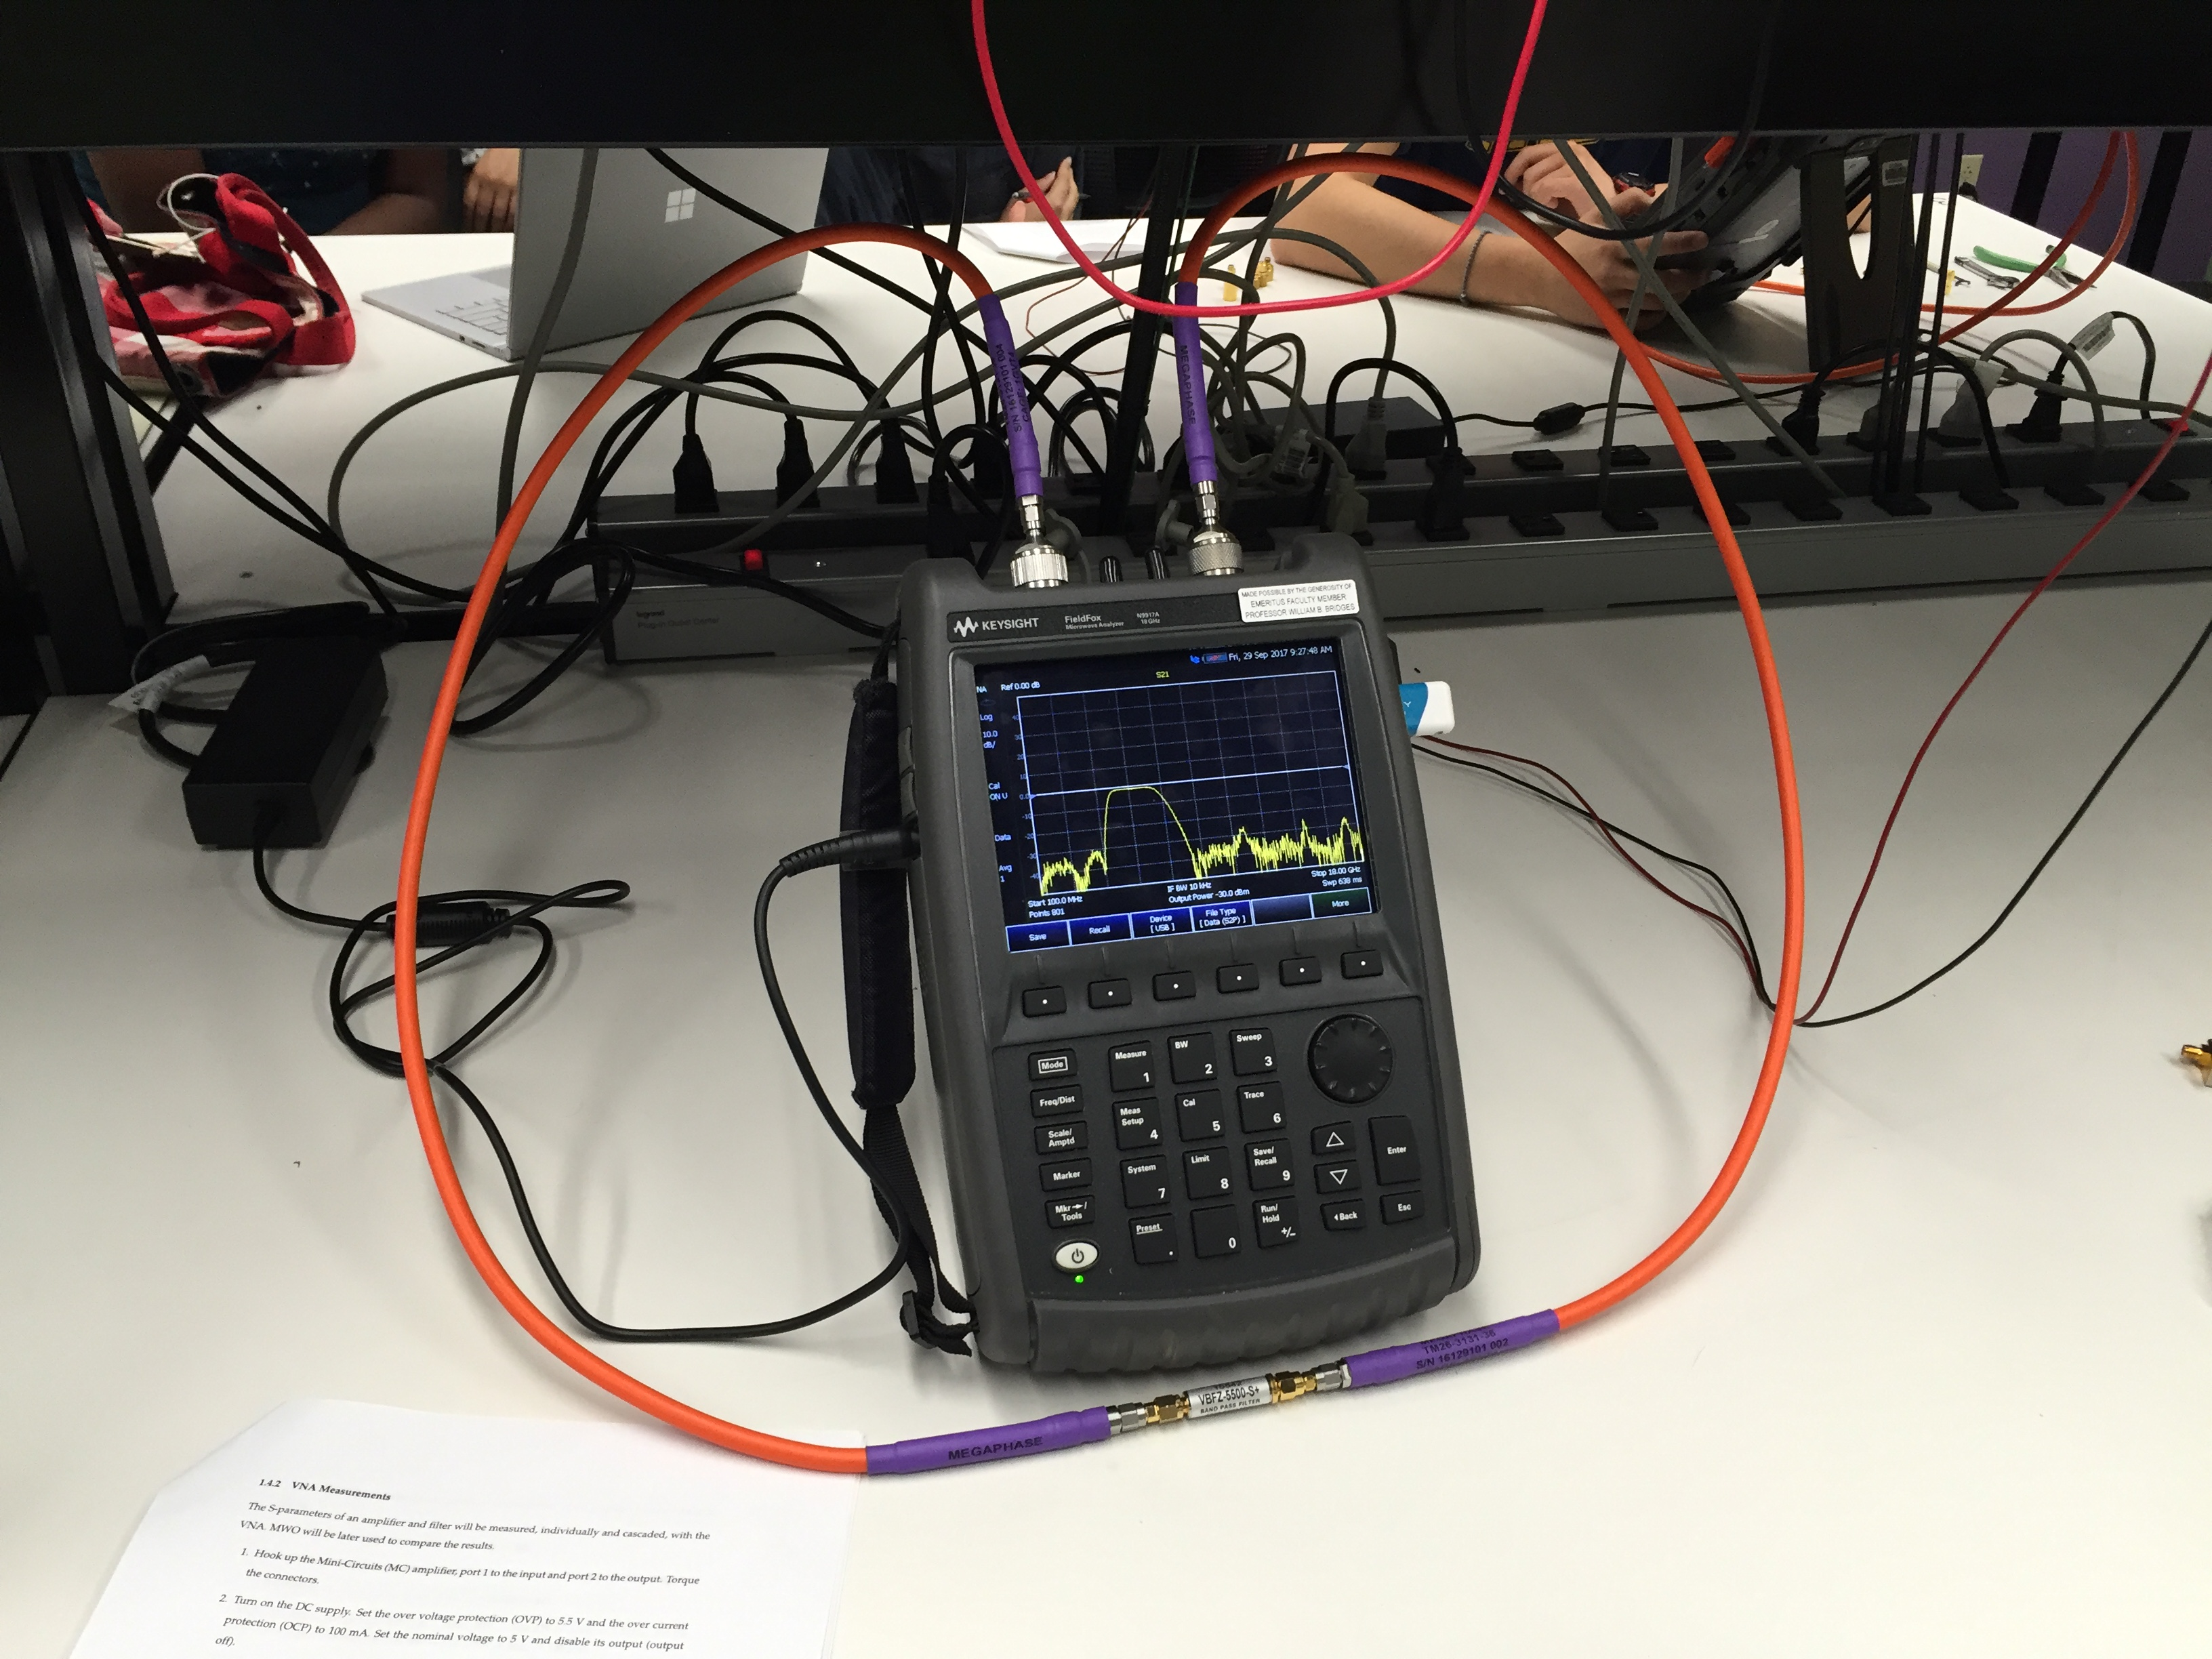
\includegraphics[width=0.35\textwidth]{filter_measurement.jpeg}
%     \caption{Measurement Setup for filter on the NA.}
%     \label{fig:filterimg}
% \end{figure}


% \begin{figure}[!htbp]
%     \centering
%     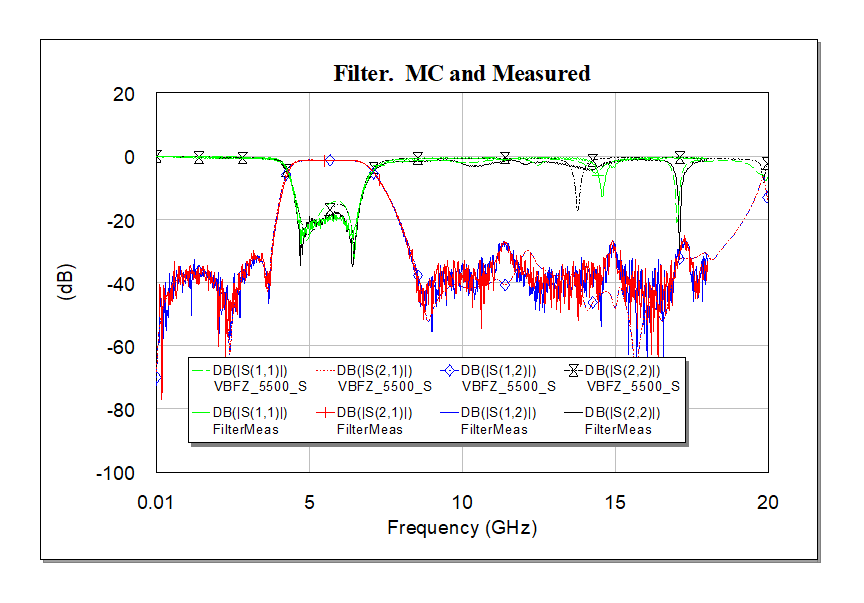
\includegraphics[scale=0.45]{FilterMCandMeasured.png}
%     \caption{Comparison of the Filter S parameters from the NA measurements to the sourced values from the data sheet.}
%     \label{fig:filter}
% \end{figure}


\FloatBarrier

\section*{Impedance Matching}

We designed a lumped element matching network for an already populated RC network on a circuit board. To do so, we first measured $S_{11}$ for the RC circuit to obtain its input impedance as a function of frequency to match it at 4 GHz. In order to make the measurement of the RC circuit S parameter, it was necessary for us to adjust the reference plane to account for the electrical delay due to the SMA connector and microstrip section that connected the RC circuit to the NA. The time delay $\tau$ at the frequency $f$ can be calculated from the electrical delay $\phi$ given as a phase angle (as is done in TXLine) using the equation $\tau = \frac{\phi}{2 \pi f}$. The coaxial line of the SMA connector was 290 mil long with a 50 mil diameter inner conductor and a 168 mil diameter outer conductor. Teflon, which fills the coax line, has a dielectric constant of 2.1 giving an electrical length of 51.27 \textdegree. The microstrip section which was 430 mil long on 12 mil thick FR-4 (dielectric constant of 4.4) had an electrical length of 95.37 \textdegree for a 20 mil wide traces that was 1.7 mils thick. Using the time delay equation and the total electrical length obtained from TXLine, we obtained the total time delay of the circuit as 101.8 ps. This was the value used to move the reference plane of the VNA to the plane of the RC network.

The matching network was designed in MWO using a Smith Chart to achieve a match with a 50 $\Omega$ line at 4 GHz. 


In order to correctly measure the input power vs. output power response of the MC amplifier, we needed to first quantify the losses in the circuit due to the cabling and connectors. To do so, we connected a signal generator through the SMA cables to the SA and measured the power in the SA as a function of the power from the signal generator. We swept Pin from -20.0 dBm to 0.0 dBm in 1 dB steps. The results are shown in figure . This shows that we have about 2dB loss due to the cables.

% \begin{figure}[!htbp]
%     \centering
%     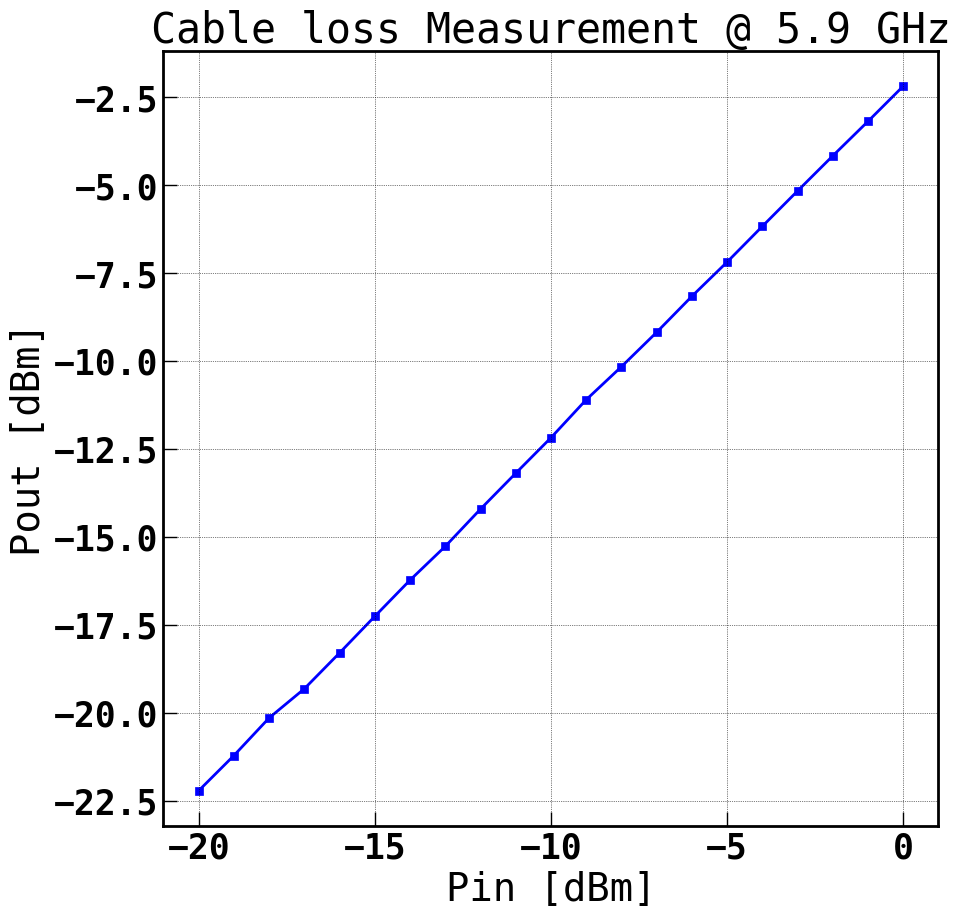
\includegraphics[scale=0.35]{cable_power_loss.png}
%     \caption{Measurements of the Input Power from signal generator to the actual power measured. This shows the power loss in the cables and connectors.}
%     \label{fig:cableloss}
% \end{figure}

Once the amplifier is connected in the circuit as shown in figure, we measured the output power of the amplifier as a function of the input power from the signal generator, adjusted for losses in the cables. In addition, a 10dB attenuator was added to the output of the amplifier to protect the SA from damage. This value was added back to the power measured by the SA. The signal generator provided a single tone at 5.9 GHz. At low input powers, the response of the amplifier is mostly linear as is shown in figure fig:ampcompress}. At higher input power, the amplifier saturates and delivers less power at 5.9 GHz than the expected linear response. This deviation is due to non-linearities becoming more and more important in the amplifier. From this, we measured the 1dB compression point of the amplifier as at an output power of 10.9 dBm at 5.9 GHz. The datasheet reports a 1dB compression point of 12.1 dBm at 6.00 GHz in contrast.

% \begin{figure}[!htbp]
%     \centering
%     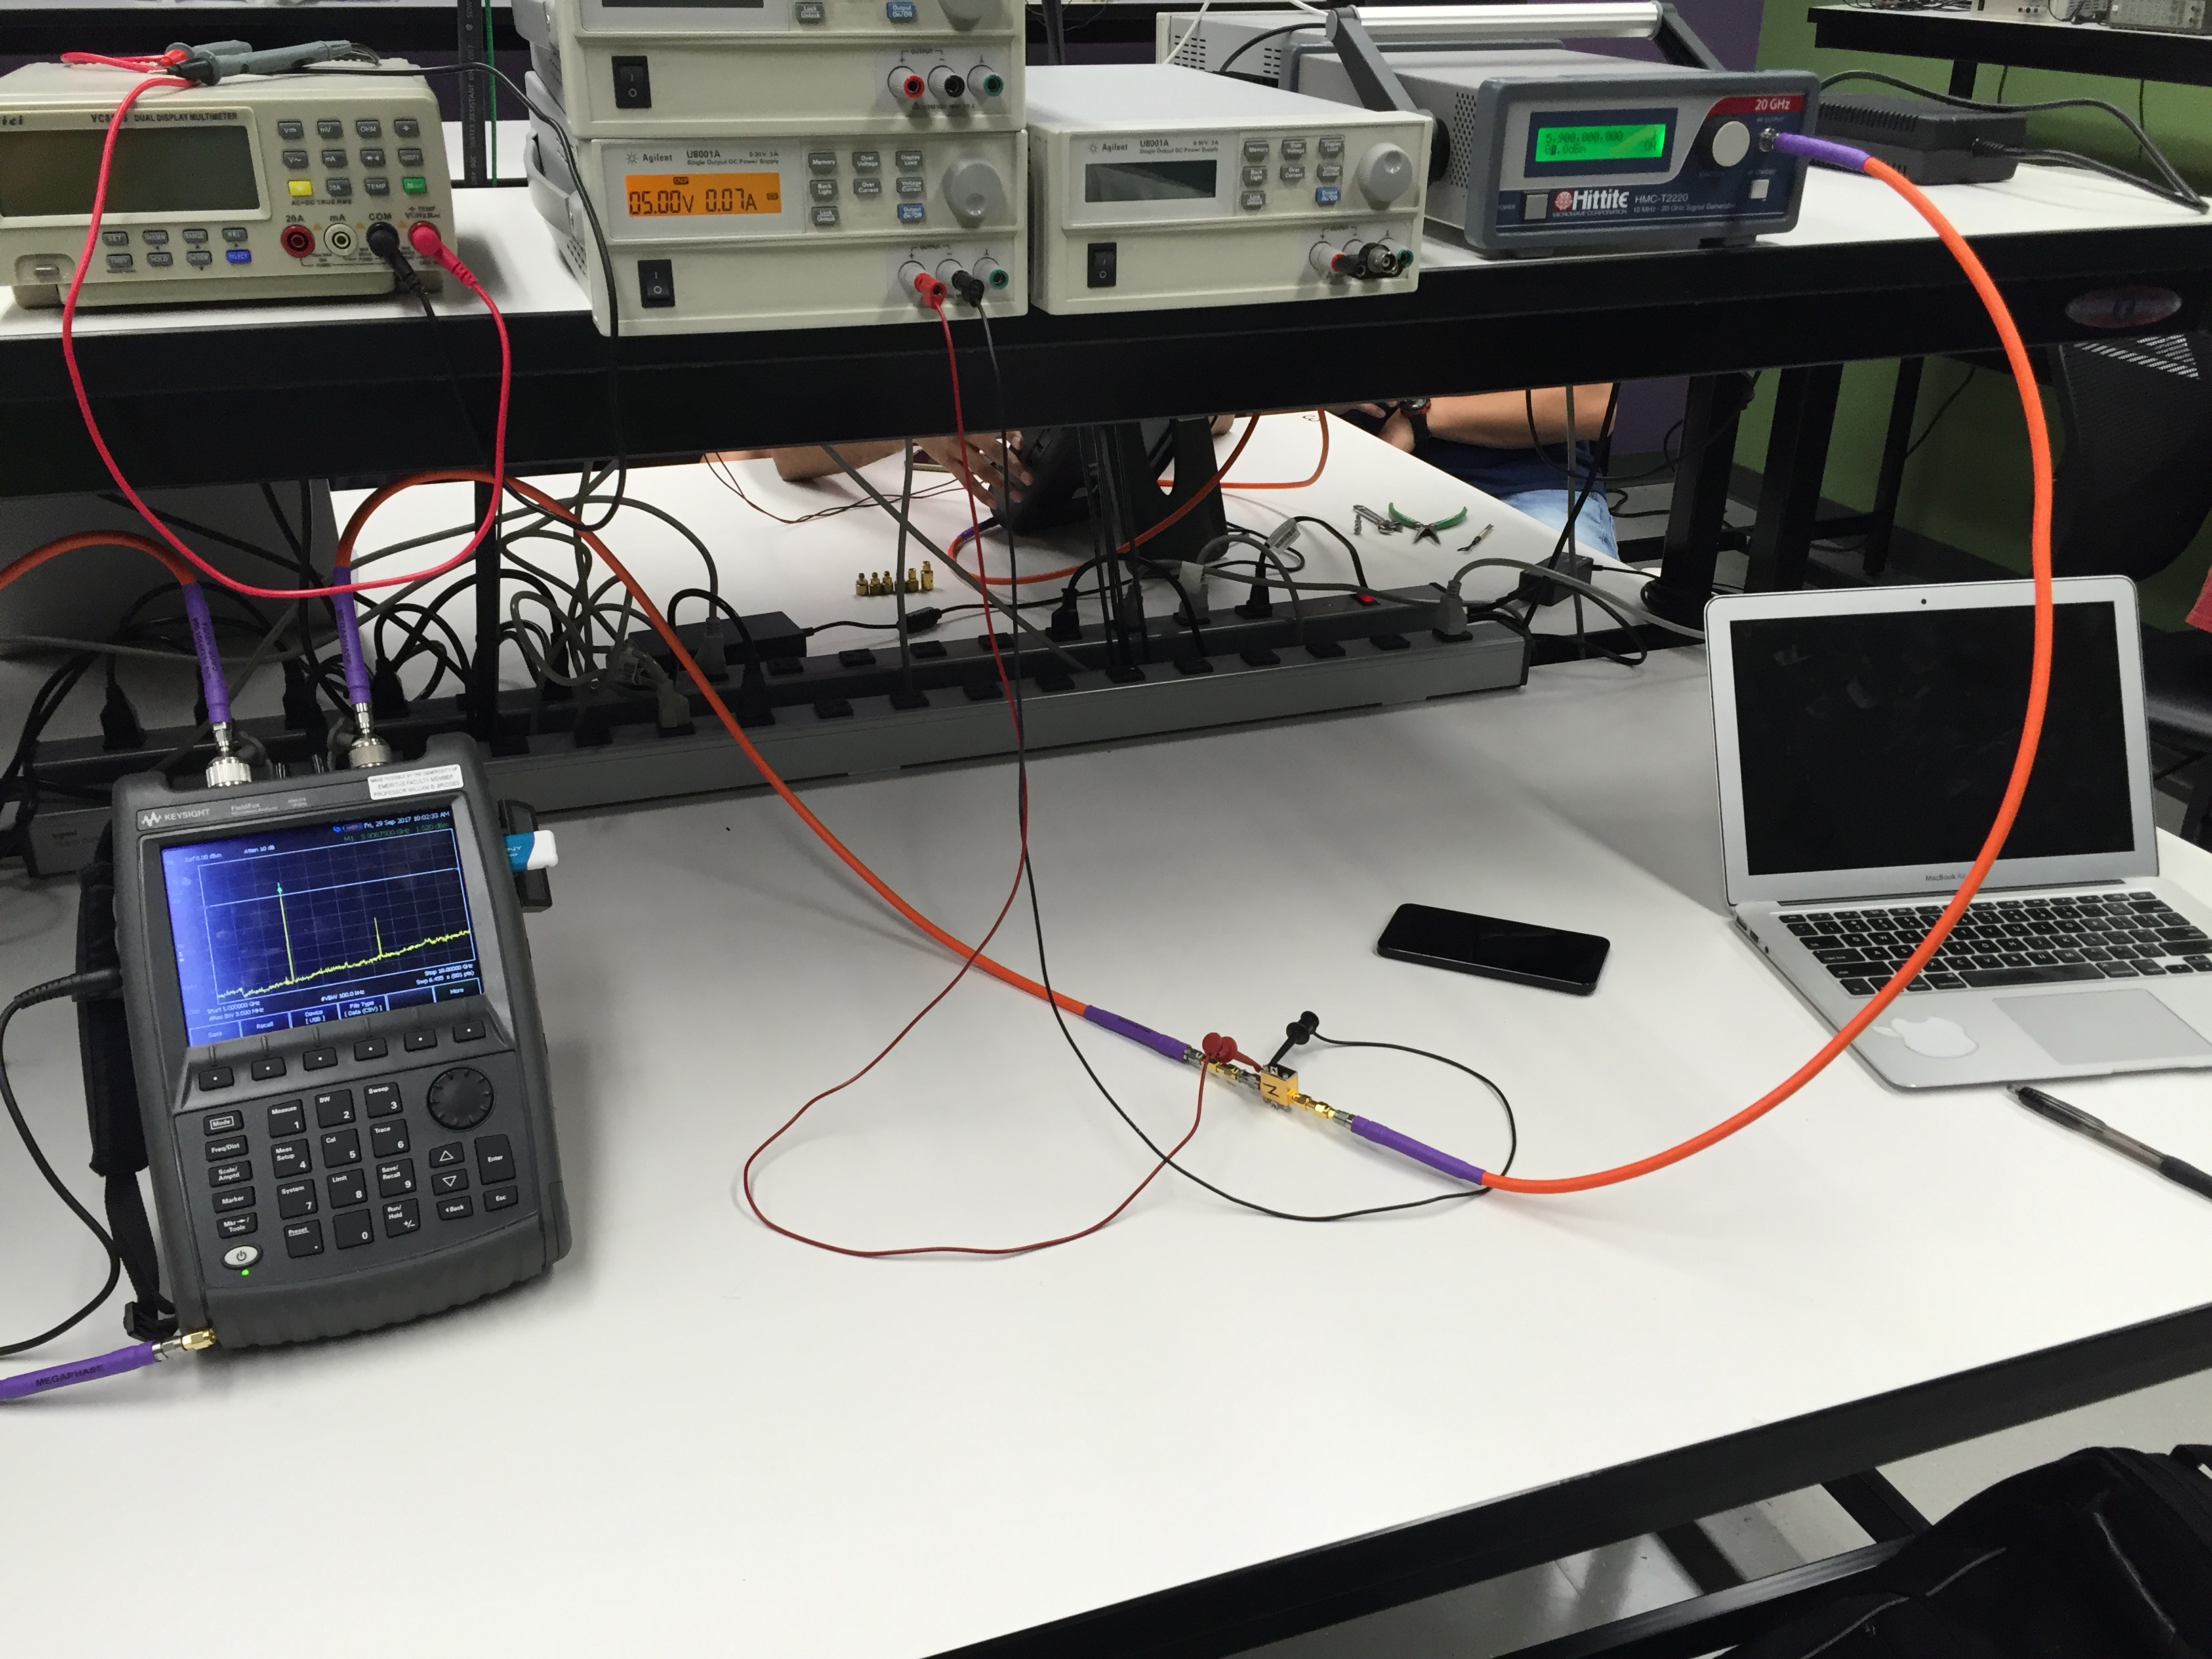
\includegraphics[width=0.35\textwidth]{amp_spectral_measurement.jpeg}
%     \caption{Measurement Setup for amplifier on the SA. The fundamental and first harmonic are visible in the SA display.}
%     \label{fig:ampspectralimg}
% \end{figure}

% \begin{figure}[!htbp]
%     \centering
%     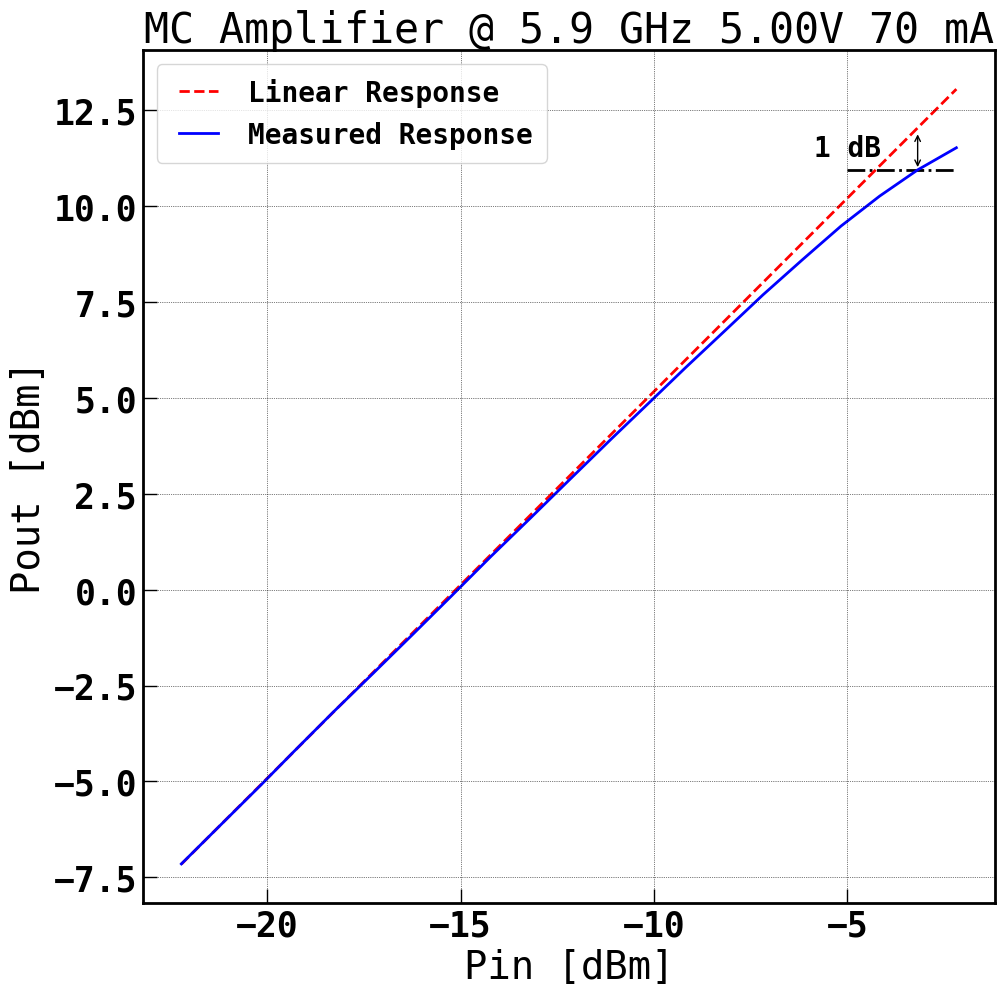
\includegraphics[scale=0.35]{amp_power_compression.png}
%     \caption{Amplifier power response. The linear response over the entire input power range has also been plotted for comparison.}
%     \label{fig:ampcompress}
% \end{figure}

As described in the introduction section, the drop in response is due to the excitation of higher order harmonics that move power away from the fundamental. This can be clearly seen in the spectral traces of the amplifier at input power of -20.0 dBm vs. 0.0 dBm as shown in figure. At low input power, only the fundamental tone is visible above the noise floor and at high SNR. At higher input power levels the second harmonic at 11.8 GHz is also clearly visible above the noise floor of the instrument.

% \begin{figure}[!htbp]
%     \centering
%     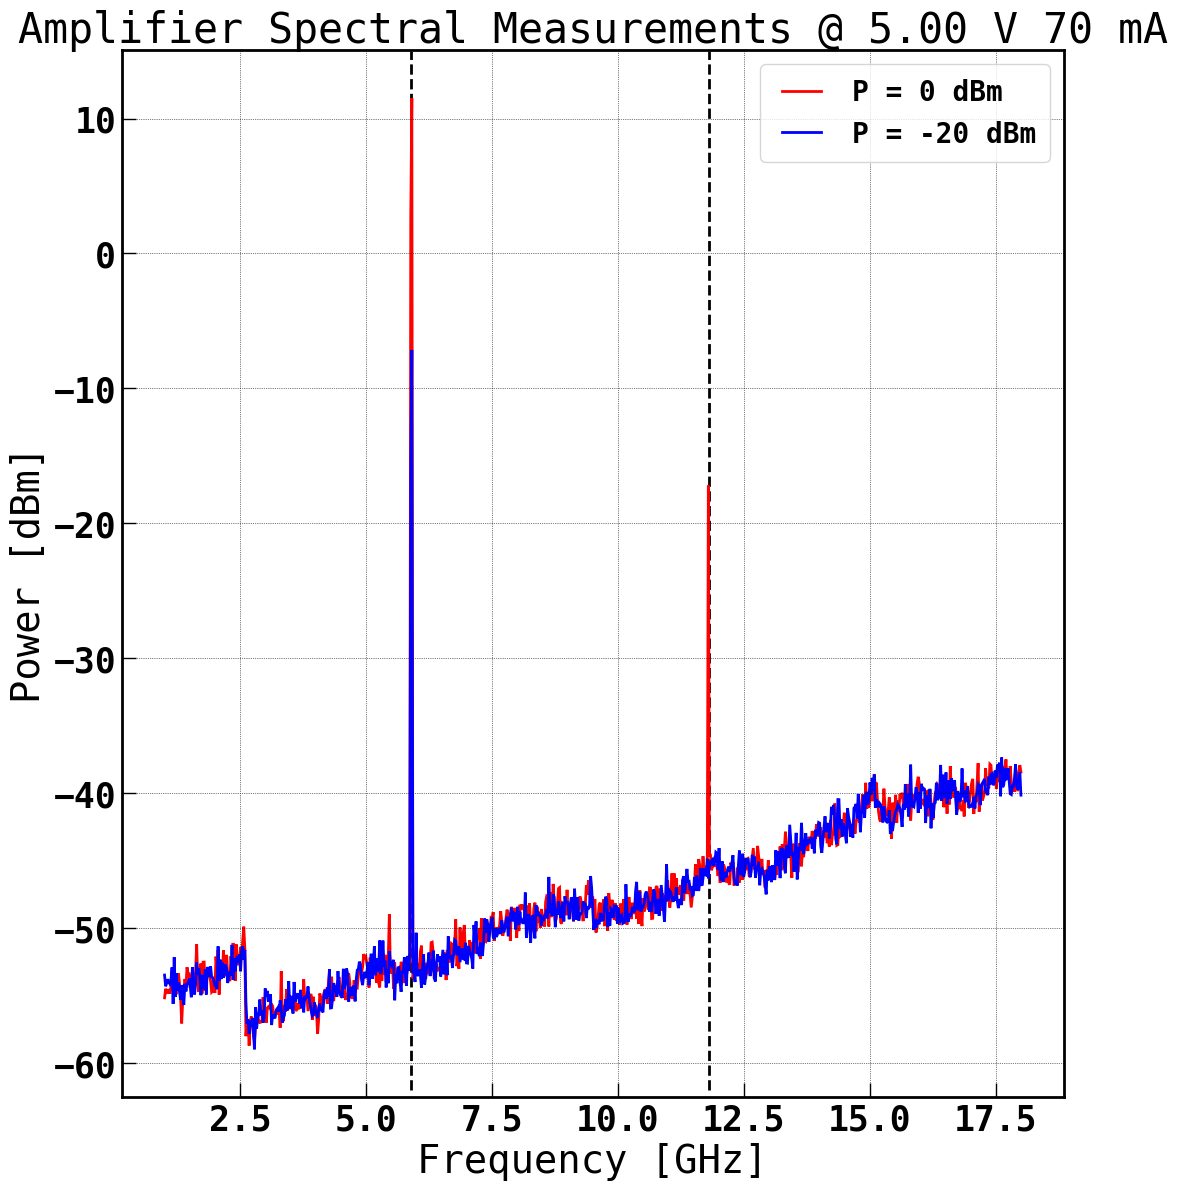
\includegraphics[scale=0.30]{spectra_20dB_vs_0dB.png}
%     \caption{A plot of the amplifier spectrum with Pin = -20.0 dBm vs 0.0 dBm. The fundamental harmonic is at 5.9 GHz. At 0.0 dBm, the first harmonic at 11.8 GHz is visible.}
%     \label{fig:spectra}
% \end{figure}

\section*{Conclusions}
At the end of this document, I have also attached the code used to generate the plots for the SA measurements. The biggest takeaways from this lab were the fundamentals of using a Network Analyzer to perform measurements of the S parameters. I learned how to interpret the NA results and compare them with datasheet specifications using Microwave Office. I also learned how to chain different S parameter files to simulate the combined response of the total network. The use of Spectral Analyzers to investigate the non-linearities of amplifiers was also a key aspect of this lab. My suggestion for improvement would be better guidance on exactly what is expected in the lab reports. I spent a lot of time writing this one up.
\end{document}